\addcontentsline{toc}{chapter}{Introduzione}
\chapter*{Introduzione}
Il \textit{Machine Learning} detto anche Apprendimento Automatico nasce come diramazione dell'intelligenza artificiale e sta prendendo sempre più piede nel mondo odierno.  
In passato questa disciplina era limitata dall'hardware disponibile, ma ora grazie all'avvento di \ac{gpu} sempre più potenti o addirittura hardware dedicato
si riesce ad usare modelli sempre più complessi e precisi in diversi ambiti della vita quotidiana. 

Il trend attuale prevede l'utilizzo sempre maggiore di Reti Neurali artificiali. Una Rete Neurale è un modello matematico che per molti versi cerca di ricalcare la funzionalità 
di un cervello umano al solo scopo di sostituirlo per quei compiti che possono essere definiti \textit{ripetitivi}. 

Il cervello umano è composto da neuroni connessi tra di loro che formano una rete, uno di questi componenti è possibile riassumerlo molto schematicamente in Figura \ref{fig:neurone}. 
\begin{figure}[]
    \centering
    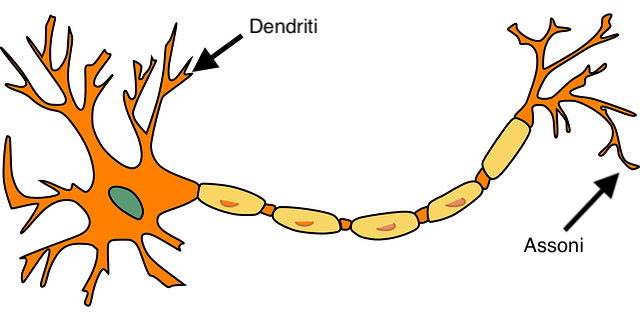
\includegraphics[width = \textwidth]{images/neurone.png}
    \caption{Schema di un neurone}
    \label{fig:neurone}
\end{figure}
All'interno di un neurone scorrono impulsi elettrici che arrivano fino all'assone, e da quest'ultimo sono modulati dalle sinapsi ed infine 
arrivano ai dendriti degli altri neuroni connessi ad esso. 
Una rete neurale artificiale, come il cervello umano è composta da tanti neuroni artificiali che sono del tutto analoghi come schema ad un neurone biologico. Hanno in input dei dati che vengono 
modulati da dei \textit{pesi} ed infine passando per una \textit{funzione di attivazione} vengono restituiti in output ad altri neuroni. 

Un esempio di utilizzo può essere la guida autonoma: sempre più case costruttrici adottano reti neurali
per realizzare veicoli sempre più sicuri e per ridurre l'intervento umano in casi di emergenza o durante lunghi viaggi, riuscendo quindi a integrare hardware molto potente in situazioni critiche. 
Lo stato dell'arte in ambito consumer sulla guida autonoma è stato raggiunto dall'americana \textit{Tesla} con il suo \textit{AutoPilot} che 
grazie a nove telecamere posizionate attorno alla vettura riesce a raggiungere un livello di autonomia mai visto prima.
Altri utilizzi possono essere la videosorveglianza, dove riconoscere intrusioni di persone o vetture all'interno di un perimetro diventa un compito critico e molto importante che fino a pochi anni fa era prerogativa solamente di esseri umani. 
Le reti neurali sono usate anche per controllo qualità, \textit{speech recognition}, \textit{sentiment analysis} e via discorrendo. 


Il nostro interesse sarà focalizzato sul miglioramento del riconoscimento su immagini che fanno parte dello spettro termico in quanto offrono un vantaggio in condizioni di scarsa visibilità rispetto alle immagini tradizionali.

Il resto dell'elaborato è strutturato come segue:
\begin{itemize}
    \item nel Capitolo 1 è stata data un introduzione all'argomento riguardante la rilevazione di oggetti, fornendo una panoramica delle metodologie, tecniche e modelli più importanti e di come si sono evolute nel corso del tempo. 
    \item all'interno Capitolo 2 si parlerà di come è stato organizzato il sistema su cui abbiamo lavorato per lo sviluppo della tesi, in particolare si affronterà da un punto di vista più descrittivo i dataset e le tecniche utilizzate. 
    \item il Capitolo 3 riguarda invece gli esperimenti effettuati usando come base ciò che è stato descritto nel precedente capitolo. 
\end{itemize}